\documentclass[pdf]{beamer}

\mode<presentation>{
  \usetheme{Singapore}          % others: default Singapore Warsaw
  \usecolortheme{dolphin}       % beetle beaver orchid whale dolphin
  \setbeamertemplate{sections/subsections in toc}[ball unnumbered]  % others: circle ball square
	\usepackage{graphicx}
  \graphicspath{ {figures/} }
  \usepackage{listings}
  \lstset{
    basicstyle=\scriptsize\color{blue}\ttfamily,
    frame=none,
    columns=l,
    tabsize=2,
    showspaces=false,
    showtabs=false
  }
  \usepackage{array}
  \hypersetup{
    colorlinks=true,
    allcolors=blue
  }
  \usepackage[edges]{forest}
  \usepackage{multicol}
}

% preamble
\title{Ansible Filters}
\subtitle{a short introduction}
\author{Frank Jung}
\institute{frankhjung@linux.com}
\date{\today}
\logo{
\includegraphics[height=1.5cm]{logos.png}}

\begin{document}

\begin{frame}
  \titlepage{}
\end{frame}

% \begin{frame}{Contents}
%   \tableofcontents{}
% \end{frame}

\section{Topics}

\begin{frame}
  \frametitle{Topics}
  What we will cover \ldots
  \pause{}
  \setbeamercolor{alerted text}{fg=blue}
  \begin{itemize}[<+-|alert@+>]
    \item what are Ansible filters?
    \item some typical use cases
    \item getting help
    \item how to roll my own?
  \end{itemize}
\end{frame}

\section{What are Ansible Filters?}

\begin{frame}
  \frametitle{What are Ansible Filters?}
  Filters are from a fast, flexible, Python template engine called \ldots
  \pause{}
  \begin{center}
    \begin{figure}
      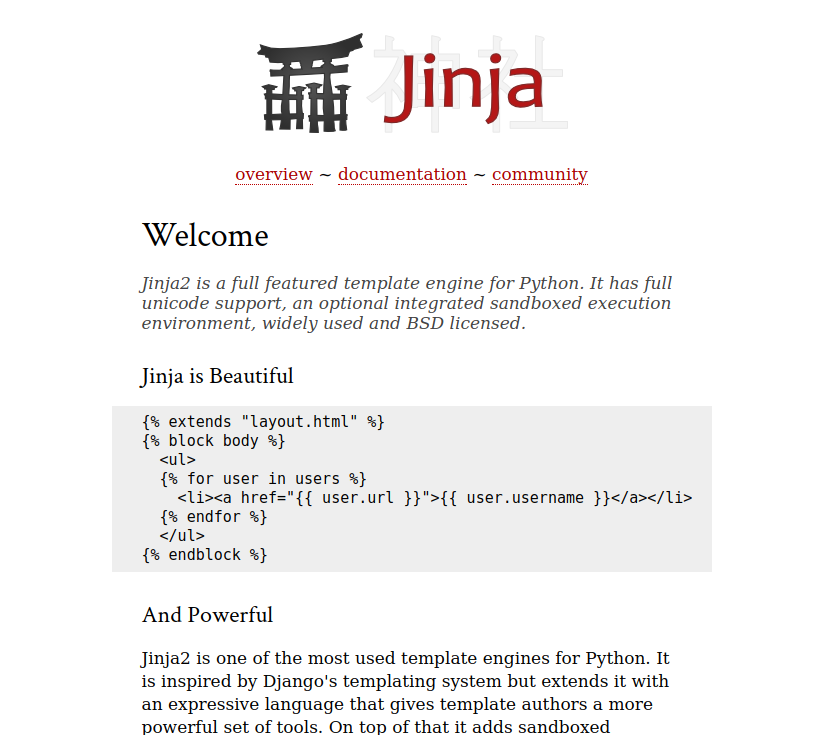
\includegraphics[width=0.5\textwidth]{jinja.png}
    \end{figure}
    \href{http://jinja.pocoo.org}{jinja.pocoo.org}
  \end{center}
\end{frame}

\begin{frame}
  \frametitle{What are Ansible Filters?}
  Filters are used to transform data \ldots
  \pause{}
  \setbeamercolor{alerted text}{fg=blue}
  \begin{enumerate}
    \item<+-> {they can be used inside a template expression}
    \item<+-|alert@+(1)> {they can be used to manipulate local data}
    \item[]
  \end{enumerate}
\end{frame}

\begin{frame}
  \frametitle{What are Ansible Filters?}
  Some important features of filters \ldots
  \pause{}
  \setbeamercolor{alerted text}{fg=blue}
  \begin{enumerate}[<+-|alert@+>]
    \item  sand boxed
      \begin{itemize}[<+-|alert@+>]
        \item so can be used to evaluate untrusted code
      \end{itemize}
    \item they are executed on the Ansible controller
      \begin{itemize}[<+-|alert@+>]
        \item \textcolor{red}{\textbf{not}} on the task's target host
      \end{itemize}
    \item Ansible ships with its own filters
      \begin{itemize}[<+-|alert@+>]
        \item or use standard filters from Jinja2
        \item or write your own!
      \end{itemize}
  \end{enumerate}
\end{frame}

\section{Typical Use Cases}

\begin{frame}[t,fragile]{Typical Filter Use Cases}
  Use filters to manipulate local data \ldots \pause
  \setbeamercolor{alerted text}{fg=blue}
  \begin{itemize}
    \item<+-|alert@+> create new facts
      \only<2> {\lstinputlisting[firstline=34,lastline=36]{filter-examples.yaml}}
    \item<+-|alert@+> subset or filter lists
      \only<3> {\lstinputlisting[firstline=52,lastline=62]{filter-examples.yaml}}
    \item<+-|alert@+> manipulate strings
      \only<4> {\lstinputlisting[firstline=87,lastline=99]{filter-examples.yaml}}
  \end{itemize}
\end{frame}

\begin{frame}[t,fragile]{Method Call}
  Python's \href{https://docs.python.org/2/library/string.html}{string
  operations} can be called \ldots
  \pause
  \begin{lstlisting}
- debug:
    msg: "{{ martin.name.upper() }}"
  \end{lstlisting}
  \pause
  Which results in \ldots
  \begin{lstlisting}
TASK [debug] **************************************
ok: [localhost] => {
    "msg": "MARTIN D'VLOPER"
}
  \end{lstlisting}
  This is the same as the Jinja's \texttt{upper} filter.
\end{frame}

\begin{frame}[t,fragile]{Pipe}
  Filters however, require to be piped \ldots
  \pause
  \begin{lstlisting}
- debug:
    msg: "{{ martin.name | hash }}"
  \end{lstlisting}
  \pause
  Which results in \ldots
  \begin{lstlisting}
TASK [debug] **************************************
ok: [localhost] => {
    "msg": "77844c7c15c84f66aa6ada7c6e2761f4aecd52c0"
}
  \end{lstlisting}
  \pause
  Using a method call will fail with \ldots
  \begin{lstlisting}[basicstyle=\scriptsize\color{red}\ttfamily]
The error was: 'ansible.parsing.yaml.objects.AnsibleUnicode
object' has no attribute 'hash'.
  \end{lstlisting}
\end{frame}

\section{Help}

\begin{frame}[fragile]
  \frametitle{Getting help when things go wrong}
  New in Ansible 2.3 is {\color{blue} \verb type_debug }:
  \begin{lstlisting}
- name: type_debug var
  debug:
    msg: "{{ martin | type_debug }}"
  \end{lstlisting}
  \pause
  Gives variable type information \dots
  \begin{lstlisting}
TASK [type_debug var] *************************
ok: [localhost] => {
    "msg": "dict"
}
  \end{lstlisting}
\end{frame}

\begin{frame}[fragile]
  \frametitle{Getting help when things go wrong}
  Ansible Project - Google Groups
  \begin{center}
    \begin{figure}
      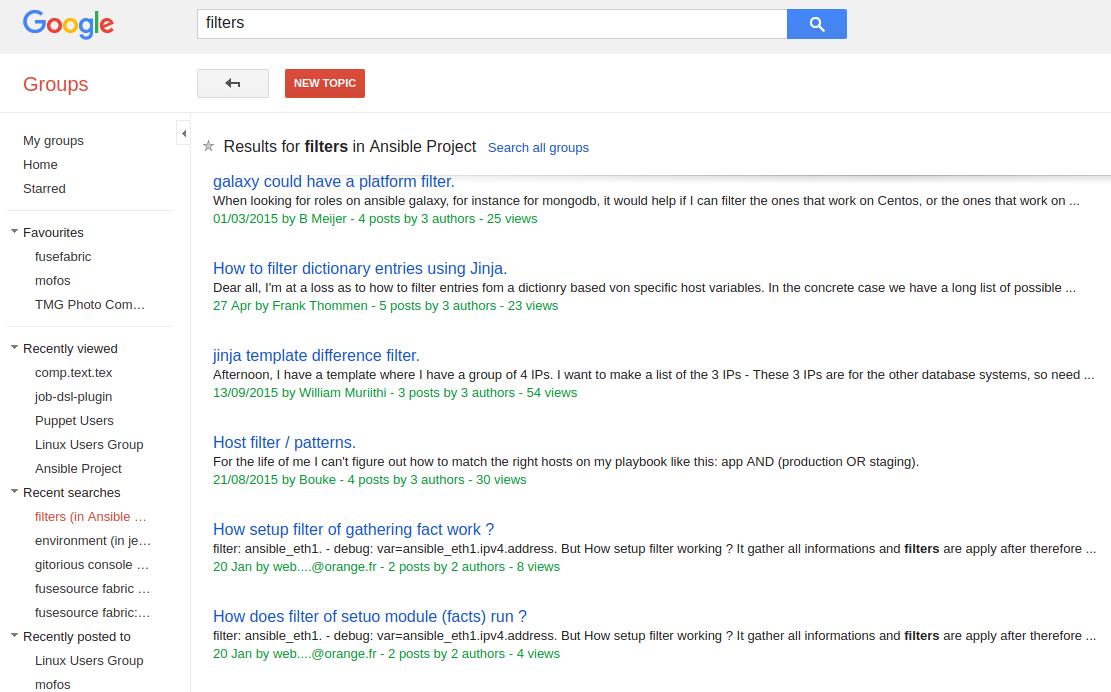
\includegraphics[width=0.8\textwidth]{ansible-google-group.png}
    \end{figure}
  \end{center}
  \tiny \url{https://groups.google.com/d/forum/ansible-project}
\end{frame}

\begin{frame}[t,fragile]
  \frametitle{Getting help when things go wrong}
  Read the source, for example Jinja has a sort method:
  \begin{lstlisting}
def do_sort(environment, value, reverse=False,
            case_sensitive=False, attribute=None):
    """Sort an iterable.  Per default it sorts ascending,
    if you pass it true as first argument it will reverse
    the sorting.
    ...
  \end{lstlisting}
  \pause{}
  Where {\color{blue}\texttt{do\_sort}} maps to \ldots \pause {\color{blue}\texttt{sort}}:
  \begin{lstlisting}
FILTERS = {
    'sort':                 do_sort,
  ...
}
  \end{lstlisting}
  \pause{}
  Which gives a hint on how to use this method:
  \begin{lstlisting}
- name: sort skills
  debug:
    var: item
  with_items: "{{ martin.skills | sort(reverse=True) }}"
  \end{lstlisting}
  \tiny \url{https://github.com/pallets/jinja/blob/master/jinja2/filters.py}
\end{frame}

\section{Roll Your Own}

\begin{frame}
  \frametitle{Writing your own filter}
  You may think to start with the Ansible documentation \ldots
  \begin{itemize}
    \item \href{http://docs.ansible.com/ansible/dev_guide/developing_plugins.html}{Ansible dev guide to developing plugins}
  \end{itemize}
  \pause
  But, that only redirects you to \ldots
  \begin{itemize}
    \item \href{https://github.com/ansible/ansible/blob/devel/lib/ansible/plugins/filter/core.py}{lib/ansible/plugins/filter}
  \end{itemize}
  \pause
  A better place to start is \ldots
  \begin{itemize}
    \item \href{http://www.dasblinkenlichten.com/creating-ansible-filter-plugins/}{Creating your own Ansible filter plugins}
  \end{itemize}
  \bigskip
  \pause
  \textit{Let's go through an example in detail \ldots}
\end{frame}

\begin{frame}[t,fragile]
  \frametitle{Writing your own filter}
  The steps to create a custom filter are \ldots
  \setbeamercolor{alerted text}{fg=blue}
  \begin{itemize}[<+-|alert@+>]
    \item {write a test for your plugin}
    \item {create a directory called \color{blue}{\texttt{filter\_plugins}}}
    \item {add a Python script into this directory, to this script \ldots}
      \begin{itemize}
        \item {add a function implementing your filter}
        \item {implement class \textcolor{blue}{\texttt{FilterModule}} overriding \textcolor{blue}{\texttt{filters}} method}
      \end{itemize}
    \item {run test on your new filter}
  \end{itemize}
  \bigskip
  \only<7>{\textit{Now the code \ldots}}
\end{frame}

\begin{frame}[t,fragile]
  \frametitle{Writing your own filter}
  Writing a custom filter in detail \ldots
  \setbeamercolor{alerted text}{fg=blue}
  \begin{itemize}
    \item<+-|alert@+> write a test for your plugin \texttt{filter-examples.yaml}
      \begin{onlyenv}<1> % code inline to remove leading spaces
        \begin{lstlisting}
- name: count number of occurrences of 'r' in name
  set_fact:
    counter: "{{ martin.name | count('r') }}"

- name: test there are exactly 2 occurrences
  assert:
    that: counter | int == 2
    msg: "expect counter to be 2 got {{ counter }}"
        \end{lstlisting}
      \end{onlyenv}
    \item<+-|alert@+> create a directory called \texttt{filter\_plugins}
      \only<2> {\newline \lstinline{mkdir filter_plugins}}
    \item<+-|alert@+> add a Python script into this directory, to this script \ldots
      \only<3> {\newline \lstinline{touch filter_plugins/custom.py}}
      \begin{itemize}
        \item<+-|alert@+> add a function implementing your filter
          \only<4> {\lstinputlisting[firstline=3,lastline=5]{filter_plugins/custom.py}}
        \item<+-|alert@+> implement class \texttt{FilterModule} overriding \texttt{filters} method
          \only<5> {\lstinputlisting[firstline=7,lastline=10]{filter_plugins/custom.py}}
      \end{itemize}
    \item<+-|alert@+> run test of your new filter
  \end{itemize}
\end{frame}

\begin{frame}[fragile]
  \frametitle{Writing your own filter}
  Ansible project structure with filters \ldots
  \color{blue}
  \begin{center}
    \begin{forest}
      for tree={%
        folder,
        grow'=0,
        fit=band,
      }
      [.
        [ansible.cfg]
        [filter-examples.yaml]
        [filter\_plugins
          [custom.py]
        ]
        [hosts]
        [README.md]
      ]
    \end{forest}
  \end{center}
\end{frame}

\section{Summary}

\begin{frame}
  \frametitle{What we covered \ldots}
  \pause{}
  \setbeamercolor{alerted text}{fg=blue}
  \begin{itemize}[<+-|alert@+>]
    \item{what filters are}
    \item{typical places you will use them}
    \item{getting help when things go wrong}
    \item{writing your own filter}
  \end{itemize}
\end{frame}

\begin{frame}
  \frametitle{List of Ansible Filters}
  \tiny
  \setlength{\columnseprule}{0mm}
  \setlength{\columnsep}{0mm}
  \begin{multicols*}{5}
    \begin{itemize}
      \item[] b64decode
      \item[] b64encode
      \item[] basename
      \item[] bool
      \item[] change
      \item[] changed
      \item[] checksum
      \item[] combine
      \item[] comment
      \item[] dirname
      \item[] expanduser
      \item[] extract
      \item[] failed
      \item[] failure
      \item[] fileglob
      \item[] from\_json
      \item[] from\_yaml
      \item[] groupby
      \item[] hash
      \item[] mandatory
      \item[] md5
      \item[] password\_hash
      \item[] quote
      \item[] random
      \item[] realpath
      \item[] regex\_escape
      \item[] regex\_findall
      \item[] regex\_replace
      \item[] regex\_search
      \item[] relpath
      \item[] sha1
      \item[] shuffle
      \item[] skip
      \item[] skipped
      \item[] splitext
      \item[] strftime
      \item[] succeeded
      \item[] success
      \item[] ternary
      \item[] to\_datetime
      \item[] to\_json
      \item[] to\_nice\_json
      \item[] to\_nice\_yaml
      \item[] to\_uuid
      \item[] to\_yaml
      \item[] type\_debug
      \item[] win\_basename
      \item[] win\_dirname
      \item[] win\_splitdrive
    \end{itemize}
  \end{multicols*}
\end{frame}

\begin{frame}
  \frametitle{List of Jinja Filters}
  \scriptsize
  \begin{multicols*}{4}
    \begin{itemize}
      \item[] abs
      \item[] attr
      \item[] batch
      \item[] capitalize
      \item[] center
      \item[] default
      \item[] dictsort
      \item[] escape
      \item[] filesizeformat
      \item[] first
      \item[] float
      \item[] forceescape
      \item[] format
      \item[] groupby
      \item[] indent
      \item[] int
      \item[] join
      \item[] last
      \item[] length
      \item[] list
      \item[] lower
      \item[] map
      \item[] pprint
      \item[] random
      \item[] reject
      \item[] rejectattr
      \item[] replace
      \item[] reverse
      \item[] round
      \item[] safe
      \item[] select
      \item[] selectattr
      \item[] slice
      \item[] sort
      \item[] string
      \item[] striptags
      \item[] sum
      \item[] title
      \item[] trim
      \item[] truncate
      \item[] upper
      \item[] urlencode
      \item[] urlize
      \item[] wordcount
      \item[] wordwrap
      \item[] xmlattr
    \end{itemize}
  \end{multicols*}
\end{frame}

\section{Addenda}

\begin{frame}
  \frametitle{Resources}
  \begin{itemize}
    \item[] Presentation and sample code
      \begin{itemize}
        \item \scriptsize \url{https://github.com/frankhjung/ansible-filters}
      \end{itemize}
    \item[] www.ansible.com
      \begin{itemize}
        \item \scriptsize \url{http://docs.ansible.com/ansible/playbooks_filters.html}
        \item \scriptsize \url{https://github.com/ansible/ansible}
      \end{itemize}
    \item[] Ansible Project - Google Groups
      \begin{itemize}
        \item \scriptsize \url{https://groups.google.com/d/forum/ansible-project}
      \end{itemize}
    \item[] Creating your own Ansible filter plugins
      \begin{itemize}
        \item \scriptsize \url{http://www.dasblinkenlichten.com/creating-ansible-filter-plugins/}
      \end{itemize}
    \item[] jinja.pocoo.org
      \begin{itemize}
        \item \scriptsize \url{http://jinja.pocoo.org/}
        \item \scriptsize \url{http://jinja.pocoo.org/docs/2.9/templates}
        \item \scriptsize \url{https://github.com/pallets/jinja}
      \end{itemize}
  \end{itemize}
\end{frame}

\begin{frame}
  \frametitle{Addendum}
  \begin{tabular}{ m{1cm} m{6cm} }
    
\includegraphics[width=1.0cm]{ansible-logo.png} & Ansible \\
    
\includegraphics[width=1.0cm]{acm-logo.png} & Association for Computing Machinery \\
    
\includegraphics[width=1.0cm]{thelinuxfoundation-logo.png} & The Linux Foundation \\
    
\includegraphics[width=1.0cm]{themarlogroup-logo.png} & The Marlo Group
  \end{tabular}
\end{frame}

\begin{frame}{}
  \begin{center}
    \Large{\insertauthor} \par
    \large{\insertinstitute} \par
    \large{\url{github.com/frankhjung/ansible-filters}}
  \end{center}
\end{frame}

\end{document}
